% This is a template for BU-ECE Technical Report.
%
% Depending on report content and author preference, a BU-ECE report may be
% in one of the two following styles:
%
%   - genuine report based on ``report'' style, i.e., with chapters, much like
%     a thesis; can be single- or double-sided,
%
%   - report based on ``article'' style, i.e., with no chapters (only sections,
%     subsections, etc.), much like a journal or conference paper; can be
%     single- or double-sided.

% =====================================================================

%\documentclass[12pt]{report}          %Single-sided report style (chapters)
%\documentclass[12pt,twoside]{report}  %Double-sided report style (chapters)
\documentclass[12pt]{article}         %Single-sided article style (no chapters)
%\documentclass[12pt,twoside]{article} %Double-sided article style (no chapters)

\usepackage{bu_ece_report}

\usepackage{graphicx}

\usepackage{dblfloatfix}

\usepackage{makecell}

\usepackage{tikz}
\def\checkmark{\tikz\fill[scale=0.4](0,.35) -- (.25,0) -- (1,.7) -- (.25,.15) -- cycle;} 

\usepackage{colortbl,dcolumn}

% In case an adjustment of vertical or horizontal margins is needed
% due to particular LaTeX/dvips or OS installation, you can uncomment
% and edit the following definitions.
% -------------------------------------------------------------------
%\topmargin       0.00 in
%\oddsidemargin   0.50 in
%\evensidemargin  0.00 in

\begin{document}

% Definitions.
% ------------
\buecedefinitions%
        {PUCKfish Product Definition and Requirements Review}
        {PUCKfish PDRR}
        {William Aracri, Peter Ha, Ammar Hussain, Alex Necakov,\newline Victoria Thomas}
        {10/22/21}
        {2021-NN} % Number of the report (four year digits and number)
        
\pagenumbering{roman}

% Title page
% (adds an empty page in double-sided printing mode).
% ---------------------------------------------------
\buecereporttitlepage

% Table of contents, list of figures and list of tables.
% ``\bueceemptypage'' adds empty page in double-sided
% printing mode and performs ``\clearpage'' in single-sided
% mode.
% ------------------------------------------------------
\tableofcontents
\vspace{50px}
\listoffigures
\listoftables\bueceemptypage

% Switch on running headers for the report:
%   odd pages  - title (lowercase); if too long, use
%                the first few words followed by ``...'',
%   even pages - last names of the authors.
% -------------------------------------------------------
\buecereportheaders

% Report summary; max. 1 page.
% (adds an empty page in double-sided printing mode).
% ---------------------------------------------------
%\setlength\parindent{24pt}
\pagenumbering{arabic}
\setcounter{page}{1}
\buecereportsummary{There are less than 400 North American Right Whales remaining in the ocean today. Unfortunately, 34 of these endangered creatures have died of unnatural causes since 2017, and lobster trap entanglement and fishing vessel collisions are the leading causes of these deaths. Our company, Fathom Fishing, is looking for your help in developing the PUCKFish, an underwater sensor device, with the goal of eventually ridding the sea of entanglement-prone lobster-fishing lines and allowing fishermen to make fewer, more-efficient trips to their traps. The PUCKFish data collection kit consists of a base station (to be mounted on fishing vessels) and several small sensing devices (to be mounted on or near individual lobster traps). In the long term, these devices will allow fishermen to wirelessly locate and hoist their traps up from the ocean floor without needing to leave location-marking buoy lines floating where they can harm whales and other sea life. The first revision of the PUCKFish, however, will simply collect temperature, depth, dissolved oxygen, and other measurements of the water surrounding a deployed lobster trap. As soon as a fisherman pulls the trap above the surface, the PUCKFish will wirelessly upload the collected data to the onboard base station. Fishermen can then use this data to determine the locations and water conditions in which they’ll catch the biggest haul, reducing the number of trips needed to reach their legal sustainable catch limit, and marine biologists can use this data to track sea life conservation efforts.}

\twocolumn

% Following sections, subsections, etc.
% -------------------------------------
\section{Need for this Project}

\par Due to hundreds of years of overfishing and mass pollution of the oceans, the pollution of right whales has decreased drastically. Whales play an important role in the environment, keeping other eat populations in check by eating “small fish, krill, larvae, copepods, pteropods, zooplankton, cyprids, euphausiids and other small invertebrates”. \cite{whalefacts:2015} Additionally, whale populations provide an important role in reducing atmospheric carbon as their excrement is the main source of food for oxygen producing phytoplankton. \cite{sapir:2021}

\par Currently, the leading cause of death in the critically endangered North Atlantic Right Whale is “entanglements and vessel strikes.” \cite{noaa:2021} \cite{noaa:2021_2} This issue has caused legislation such as the Atlantic Coastal Fisheries Cooperative Management Act which effectively illegalizes lobster fishing in large areas of the Atlantic Coast. \cite{congress:1981} \cite{congress:1981_2} To protect these animals, lobster fishermen will have to invest in technologies which reduce lobster line pollution. One solution to this issue will be the PuckFish. As our device will provide fishermen with the information to better approximate the location of lobsters, they will be able to place fewer traps, more effectively, directly decreasing the chances of whale entanglement. 

\section{Problem Statement and Deliverables}

\subsection{Problem Statement}

\par There is a current lack of data available to lobster catchers. Existing solutions use out of date technology, and give almost none of the data critical to deciding trap placement. This leads to an overabundance of traps in areas with very little yield, leading to efficiency losses for the lobster catchers, and creating greater pollution in the form of fishing lines connecting the traps to each other and buoys. 
\par Our solution simultaneously solves each of these problems, giving trappers the data most useful in locating lobsters, including dissolved oxygen, soil softness, and temperature. By allowing lobster catchers to easily access these measurements, they can place fewer traps with greater yield. This data will then be collected to create among the most robust oceanographic databases, updated far more regularly and over a wider area than existing databases. 

\subsection{Deliverables}

A set of three sensing devices capable of: 
\begin{enumerate}
    \item Measuring:
    \begin{enumerate}
        \item Temperature
        \item Dissolved oxygen
        \item Salinity
        \item Current speed and direction
        \item Depth
        \item Ambient light
    \end{enumerate}
    \item Transmitting the Collected Data:
    \begin{enumerate}
        \item On the surface
        \item 1 MB at 50 kb/s from 50 ft away
        \item Polling rate of 1/hr - 1/min
    \end{enumerate}
\end{enumerate}

A base station capable of: 
\begin{enumerate}
    \item Receiving data at the above rates
    \item Storing data on an SD card in CSV format
    \item Withstand exposure to constant marine conditions
\end{enumerate}

\section{Visualization}  % Article style

\begin{figure}[h]
    \centering
    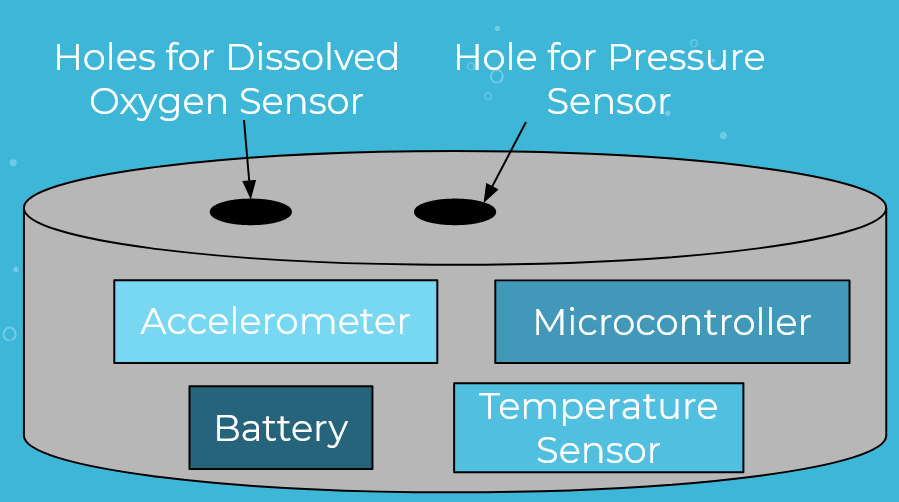
\includegraphics[scale=0.6]{puck}
    \caption{Puck, Data Collection Device}
    \label{fig:my_label}
\end{figure}

\begin{figure}[h]
    \centering
    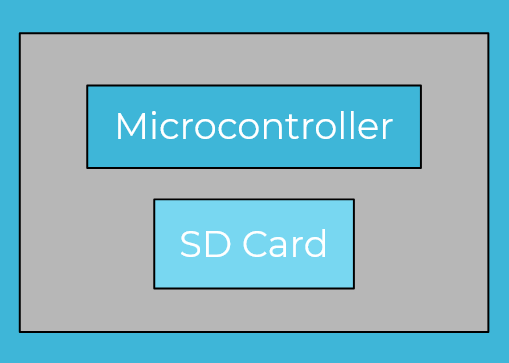
\includegraphics{fish}
    \caption{Base Station}
    \label{fig:my_label}
\end{figure}

\section{Competing Technologies}  % Article style

\begin{table*}[!b]
    \begin{center}
        \begin{tabular}{|c|c|c|c|c|c|c|c|}
            \hline
            Product & \thead{Dev. Time\\(Months)} & Temp. & \thead{Dis.\\Ox.} & Depth & Salinity & Current & \thead{Ambient\\Light} \\
            \hline
            PUCKfish & 6 & \cellcolor{green} \cellcolor{green} \checkmark & \cellcolor{green} \checkmark & \cellcolor{green} \checkmark & \cellcolor{green} \checkmark & \cellcolor{green} \checkmark & \cellcolor{green} \checkmark \\
            \hline
            \hline
            Major Competitors: & & & & & & & \\
            \hline
            TimeZero & 6 & \cellcolor{red} $\times$ & \cellcolor{green} \checkmark & \cellcolor{green} \checkmark & \cellcolor{green} \checkmark & \cellcolor{green} \checkmark & \cellcolor{red} $\times$ \\
            \hline
            eMOLT & 0 & \cellcolor{green} \checkmark & \cellcolor{red} $\times$ & \cellcolor{red} $\times$ & \cellcolor{green} \checkmark & \cellcolor{green} \checkmark & \cellcolor{red} $\times$ \\
            \hline
            \hline
            Minor Competitors: & & & & & & & \\
            \hline
            LobsterNet & 14 & \cellcolor{green} \checkmark & \cellcolor{green} \checkmark & \cellcolor{green} \checkmark & \cellcolor{red} $\times$ & \cellcolor{red} $\times$ & \cellcolor{red} $\times$ \\
            \hline
            OSU & 0 & \cellcolor{green} \checkmark & \cellcolor{green} \checkmark & \cellcolor{red} $\times$ & \cellcolor{red} $\times$ & \cellcolor{red} $\times$ & \cellcolor{red} $\times$ \\
            \hline
            \hline
            Non-Competitors: & & & & & & & \\
            \hline
            LasTrap & 0 & \cellcolor{red} $\times$ & \cellcolor{red} $\times$ & \cellcolor{red} $\times$ & \cellcolor{red} $\times$ & \cellcolor{red} $\times$ & \cellcolor{red} $\times$ \\
            \hline
            LobsterLift & 8 & \cellcolor{red} $\times$ & \cellcolor{red} $\times$ & \cellcolor{red} $\times$ & \cellcolor{red} $\times$ & \cellcolor{red} $\times$ & \cellcolor{red} $\times$ \\
            \hline
        \end{tabular}
        \caption{Competing Technologies}
        \label{tab:my_label}
    \end{center}
\end{table*}

\par The PUCKFish has competitors that the team has grouped into three separate groups as determined by their requirements and features. The first of these three groups, Non-Competitors, exhibits similar goals to PUCKFish, but does not solve these problems in a similar way that competes with PUCKFish. The second group of competitors is called Minor Competitors. Minor Competitors have projects with the same goal of measuring the environment of the Lobster trapping industry, but do not include all of the features that are unique to PUCKFish. The final group is called Major Competitors. Major Competitors include most features that PUCKFish does and have the largest weight on the requirements of our design and outline the niches that PUCKFish situates itself in.

\subsection{Major Competitors}
\subsubsection{TimeZero}
\par TimeZero is a large-scale service that provides a variety of data from all over the world.  Professional fishermen can select the services they require, although they do not collect ambient light measurements. TimeZero is a worldwide presence, which means that their focus varies and is not necessarily centralized to the Lobster industry in the northeast. PUCKFish should collect the same variety of information, while maintaining its niche with lobster nets.

\subsubsection{eMOLT}
\par eMOLT is a network of data collection equipment deployed on lobster traps. The data is collected by the fisherman community and then updated and available on a public form to see. eMOLT is the closest competitor and carries out essentially the same functions as PUCKFish. In order to improve upon this existing design, depth, ambient light, and most importantly, dissolved oxygen levels must be collected. In addition, the infrastructure and data provided must be more readily readable or translatable.

\subsection{Minor Competitors}
\subsubsection{Oregon State University Data Collection System}
\par Oregon State University developed a small micro controller to collect temperature and dissolved oxygen levels. The last update of this project was in 2009. PUCKFish must at least take temperature and dissolved oxygen levels at a depth, and do so better with more fidelity as it is newer.

\subsubsection{LobsterNet}
\par LobsterNet is a project incubated by Gloucester Innovation and powered by the Canadian company Sigfox. It collects live data in the form of temperature, oxlevel, pH, depth, and location. PUCKFish must collect at a minimum these data points. PUCKFish will not collect data live because, as shown by LobsterNet, a large infrastructure must be put into place to achieve successful implementation. LobsterNet was announced in 2019 with very little information or updates coming out since then.

\subsection{Non-Competitors}
\subsubsection{LobsterLift}
\par LobsterLift is a lobster trap that lifts itself with no lead line. This feature helps with one of the possible features of PUCKFish, but contains no sensor information relaying fisherman useful data. As a result, PUCKFish should not attempt to develop a self lifting capability until other sensor technology is implemented successfully.

\subsubsection{LasTrap}
\par LasTrap is a novel lobster trap made out of plastic leading to more resilient traps with the possibility of introducing further innovations. However, LasTrap does not include sensors, information collectors, or active components. PUCKFish is deployed on existing traps, so LasTrap does not have any impact based upon the requirements already presented.

\section{Engineering Requirements}  % Article style

PUCKfish Sensor Collection Device:
\begin{enumerate}
    \item Mechanical
    \begin{enumerate}
        \item The device must operate at 1100 ft below sea level, at pressures of over 34 atm
        \item The device must have ports for sensor access to water and user access to sensors
        \item The device must be waterproof and capable of surviving harsh, undersea conditions
    \end{enumerate}
    \item Data Collection
    \begin{enumerate}
        \item The device must collect data for the following measurements at a rate of at least one reading per hour:
        \begin{enumerate}
            \item Temperature
            \item Dissolved oxygen
            \item Salinity
            \item Current speed and direction
            \item Depth
            \item Ambient light
        \end{enumerate}
    \end{enumerate}
    \item Transmission
    \begin{enumerate}
        \item The device must detect when it has submerged/surfaced to begin transmitting to the base station
        \item Device must be able to wirelessly transmit when trap surfaces (1 MB at 50 kb/s from 50 ft away)
    \end{enumerate}
    \item Power
    \begin{enumerate}
        \item Device must be easily rechargeable, getting power from onboard lead acid marine batteries
        \item Device must last on a single charge for up to 10 days
    \end{enumerate}
    \item Cost
    \begin{enumerate}
        \item The prototype for the device must not exceed \$150, and should cost \$50 or less when produced at scale
    \end{enumerate}
\end{enumerate}

Base Station:
\begin{enumerate}
    \item Mechanical 
    \begin{enumerate}
        \item The Base Station must be able to withstand frequent splashes of saltwater, heavy rain, and other harsh marine conditions
    \end{enumerate}
    \item Data Collection
    \begin{enumerate}
        \item The Base Station must receive data as PUCKFish transmits, saving the data in CSV format
        \item The Base Station must store data on a SD card so data can be easily transferred to other systems for data analysis
    \end{enumerate}
    \item Power
    \begin{enumerate}
        \item The Base Station must be able to be powered off of onboard lead acid marine batteries, accepting voltages in anywhere in the range of 11-14V
    \end{enumerate}
\end{enumerate}

\section{Appendix A: References}  % Article style

% Bibliography.
% -------------
\parskip=0pt
\parsep=0pt
\bibliographystyle{ieeetrsrt}

% Important: substitute your BiBTeX (*.bib) files below.
% ------------------------------------------------------
\bibliography{bib.bib}

\end{document}
